\subsection{连续函数空间的可数性性质}

定理 1. 设 X 是紧空间。

\begin{enumerate}
\def\labelenumi{\alph{enumi})}
\item
  若 X 可度量化且 Y 是任一可数型的可度量化一致空间（第 IX 章，§ 2，第 8 号），则由 X 到 Y 中的连续映射所成的可度量化空间 \(\mathcal{C}_{\mathbf{u}}(\mathbf{X};\mathbf{Y})\) （赋有一致收敛拓扑）是可数型的。
\item
  反之，若可度量化空间 \(\mathcal{C}_{u}(\mathbf{X};\mathbf{R})\) 是可数型的，则 \(\mathbf{X}\) 可度量化。
\item
  设 \(d\) （相应地，\(d'\) ）是与 \(\mathbf{X}\) 的拓扑（相应地，\(\mathbf{Y}\) 的一致结构）相容的度量；则 \(\delta(f, g) = \sup_{x \in \mathbf{X}} d'(f(x), g(x))\) 是定义空间 \(\mathcal{C}(\mathbf{X}; \mathbf{Y})\) 上的一致收敛的一致结构的一个度量，\(\mathcal{C}(\mathbf{X}; \mathbf{Y})\) 中的函数是有界的，因为 \(\mathbf{X}\) 紧（第 1 号）。对每对整数 \(m > 0\) 、 \(n > 0\) ，设 \(\mathbf{G}_{mn}\) 是诸函数 \(f \in \mathcal{C}(\mathbf{X};\mathbf{Y})\) （满足关系 \(d(x,x') \leqslant 1 / m\) 蕴涵 \(d(f(x),f(x')) \leqslant 1 / n\) ）所成之集。每个函数 \(f \in \mathcal{C}(\mathbf{X};\mathbf{Y})\) 都一致连续（第 II 章，§ 4，第 1 号，定理 2），因此对每个 \(n > 0\) ，\(\mathcal{C}(\mathbf{X};\mathbf{Y})\) 是诸集 \(\mathbf{G}_{mn}(m > 0)\) 的并。设 \(\{a_1,\dots ,a_{p(m)}\}\) 是 \(\mathbf{X}\) 的一个有限子集，使得以 \(a_i\) 为中心、\(1 / m\) 为半径的开球覆盖 \(\mathbf{X}(1\leqslant i\leqslant p(m))\) ；并设 \((b_r)_{r\in \mathbb{N}}\) 是在 \(\mathbf{Y}\) 中稠密的一个可数序列。对每个映射 \(\varphi :[1,p(m)]\to \mathbf{N}\) ，设 \(\mathrm{H}_{\varphi}\) 是那些 \(f\in \mathbf{G}_{mn}\) （满足 \(d'(f(a_k),b_{\varphi (k)})\leqslant 1 / n\) 对 \(1\leqslant k\leqslant p(m)\) ）所成之集。由诸 \(b_r,\mathbf{G}_{mn}\) 的定义，诸集 \(\mathbf{H}_{\varphi}\) （对 \(\varphi \in \mathbf{N}^{p(m)}\) ）的并即为该集；设 \(\mathbf{C}_{mn}\) 是映射 \(\varphi \in \mathbf{N}^{p(m)}\) （使 \(\mathrm{H}_{\varphi}\neq \emptyset\) ）所成之集，且对每个 \(\varphi \in \mathbf{C}_{mn}\) 设 \(g_{\varphi}\) 是 \(\mathrm{H}_{\varphi}\) 的一个元素；最后，用 \(\mathrm{L}_{mn}\) 表示诸 \(g_{\varphi}\) （对 \(\varphi \in \mathbf{C}_{mn}\) ）所成的可数集。设 \(f\in \mathbf{G}_{mn}\) ，并设 \(\varphi\) 是 \(\mathbf{C}_{mn}\) 的一个元素（使 \(f\in \mathrm{H}_{\varphi}\) ）；则由定义立即得出，\(d'(f(x),g_{\varphi}(x))\leqslant 4 / n\) 对一切 \(x\in X\) 成立，即 \(\delta (f,g_{\varphi})\leqslant 4 / n\) 。因此诸集 \(L_{mn}\) 的并在 \(C_u(\mathbf{X};\mathbf{Y})\) 中稠密，因为对每个整数 \(n > 0\) 及每个 \(f\in \mathcal{C}(\mathbf{X};\mathbf{Y})\) 存在 \(m\) 使 \(f\in G_{mn}\) ，而我们刚看到 \(f\) 到 \(L_{mn}\) 的距离 \(\leqslant 4 / n\) 。
\item
  设 I = {[}0, 1{]}。由于 \(\mathcal{C}_{u}(\mathbf{X};\mathbf{I})\) 是 \(\mathcal{C}_{u}(\mathbf{X};\mathbf{R})\) 的一致子空间，它是可数型的。设 \((f_{n})\) 是在 \(\mathcal{C}_{u}(\mathbf{X};\mathbf{I})\) 中稠密的一个序列。考虑积空间 \(K=I^{N}\) 以及映射 \(\psi: x\to(f_{n}(x))\) （由 X 到 K 中），它显然连续。映射 \(\psi\) 是单射；因为由序列 \((f_{n})\) 的定义，关系 \(f_{n}(x)=f_{n}(x')\) （对一切 n）在取极限后蕴涵 \(f(x)=f(x')\) 对每个函数 \(f\in\mathcal{C}(\mathbf{X};\mathbf{I})\) 成立；但若 \(x\neq x'\) 这是不可能的，由公理 \((\mathrm{O}_{\mathrm{IV}})\) （应用于点 x 及 x 的一个不含 \(x'\) 的邻域 V）（第 IX 章，§1，第 5 号，定理 2）。由此推出，紧空间 X 同胚于 K 的子空间 \(\psi(\mathbf{X})\) （第 I 章，§9，第 4 号，定理 2 的推论 2）；由于 K 可度量化且可数型，\(\psi(\mathbf{X})\) 亦然，从而 X 亦然。
\end{enumerate}

证毕。

推论. 设 X 是拓扑具有可数基的局部紧空间，并设 Y 是可数型的可度量化一致空间。

\begin{enumerate}
\def\labelenumi{\alph{enumi})}
\item
  空间 \(\mathfrak{L}\) （由 \(\mathbf{X}\) 到 \(\mathbf{Y}\) 中且在无穷远处有极限的连续映射组成，赋有在 \(\mathbf{X}\) 中的一致收敛拓扑）是可数型的可度量化空间。
\item
  空间 \(\mathcal{C}_{c}(\mathbf{X};\mathbf{Y})\) （由 X 到 Y 中的连续映射组成，赋有紧收敛拓扑）是可数型的可度量化空间。
\item
  设 \(\mathbf{X}'\) 是由 \(\mathbf{X}\) 添加一个无穷远点所得到的紧空间（第 I 章，§ 9，第 8 号，定理 4）；按定义，每个函数 \(f \in \mathcal{L}\) 都可唯一扩张为连续函数 \(\overline{f} \colon \mathbf{X}' \to \mathbf{Y}\) ，因此 \(f \to \overline{f}\) 是 \(L\) 到 \(\mathcal{C}(X'; Y)\) 上的一个双射；而由第 1 节第 6 号的命题 6，这个双射是空间 \(L\) 到 \(\mathcal{C}_u(X'; Y)\) 上的一个同胚。由于 \(X'\) 可度量化（第 IX 章，§2，第 9 号，命题 16 的推论），把定理 1 应用于 \(X'\) 与 \(Y\) 即得结论。
\item
  设 \((\mathbf{U}_{n})\) 是 X 的一个由相对紧的开集组成的覆盖，使得 X 的每个紧子集含于某个 \(U_{n}\) （第 I 章，§ 9，第 9 号，命题 15 的推论 1）。若 S 是诸 \(\overline{U}_{n}\) 所成之集，则 C(X; Y) 上的紧收敛拓扑与 S-收敛拓扑相同。因此（第 1 节，第 2 号，注 3）空间 \(\mathcal{C}_{c}(X; Y)\) 同胚于积 \(\prod_{n}\mathcal{C}_{u}(\overline{\mathbf{U}}_{n};\mathbf{Y})\) 的一个子空间；由于每个紧空间 \(\overline{U}_{n}\) 都有可数基，它可度量化（第 IX 章，§ 2，第 9 号，命题 16）；因此每个 \(\mathcal{C}_{u}(\overline{\mathbf{U}}_{n};\mathbf{Y})\) 由定理 1 都可度量化且可数型，从而 \(\mathcal{C}_{c}(X;Y)\) 亦然。
\end{enumerate}

\pandocbounded{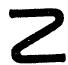
\includegraphics[keepaspectratio]{images/part002_29e6d4b6.jpg}}

注意，R 上的一切有界连续实值函数所成的空间，赋有一致收敛拓扑，不是可数型的（习题 4）。

